% day2_seg4_numerical/divergence.tex
\begin{frame}
  \onslide<1->{
	\frametitle{Filter Divergence} 
	\framesubtitle{}
}
\begin{itemize}
  \onslide<2->{
\item Kinds of Divergence
}
  \onslide<3->{
\item Causes and Remedies
}
\end{itemize}
\end{frame}

\begin{frame}
  \onslide<1->{
	\frametitle{Filter Divergence} 
	\framesubtitle{Kinds of Divergence}
}
\begin{itemize}
  \onslide<2->{
\item Mean estimation error is supposed to converge to 0
\begin{itemize}
	\item $\esterrdef$
	\item $\expect{\esterr}\rightarrow 0$
	\item Estimate is unbiased: $\expect{\hat{x}(k)}=x(k)$
\end{itemize}
}
  \onslide<3->{
\item Covariance matrix for estimation error is same as state estimation error covariance matrix: $\covmatdef$
}
\end{itemize}
\end{frame}

\begin{frame}
  \onslide<1->{
	\frametitle{Kinds of Divergence} 
	\framesubtitle{}
}
\begin{itemize}
  \onslide<2->{
\item For optimal filter, $P$ will indicate convergence or divergence.
	\begin{itemize}
		\item One common form of divergence due to round-off will send $P$ to zero
	\end{itemize}
}
  \onslide<3->{
\item For suboptimal filters, $P$ will not necessarily indicate divergence
	\begin{itemize}
	  \item $P$ may seem to indicate nominal steady-state values and yet the state estimate may go diverge from the true value
	\end{itemize}
}
\end{itemize}
\end{frame}


\begin{frame}

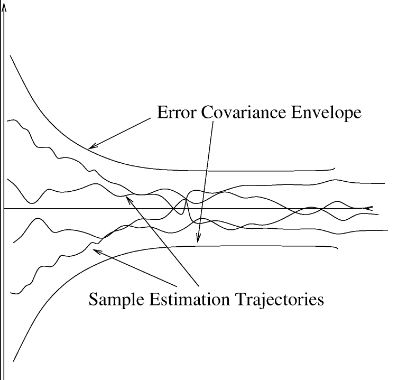
\includegraphics[scale=0.60]{day3_seg1_numerical/covconverge.jpg} 

\end{frame}


\begin{frame}
  \onslide<1->{
	\frametitle{Kinds of Divergence} 
	\framesubtitle{}
}
\begin{itemize}
  \onslide<2->{
\item Going to sleep:  error covariance becomes so small that measurements are no longer believed by the filter
}
  \onslide<3->{
\item Loss of symmetry in $P$
}
  \onslide<4->{
\item Loss of positive definiteness: negative numbers on the diagonal!
}
\end{itemize}
\end{frame}
